Artwork by Ana Cristina Chávez Cáliz.
\null
\vfill
\noindent{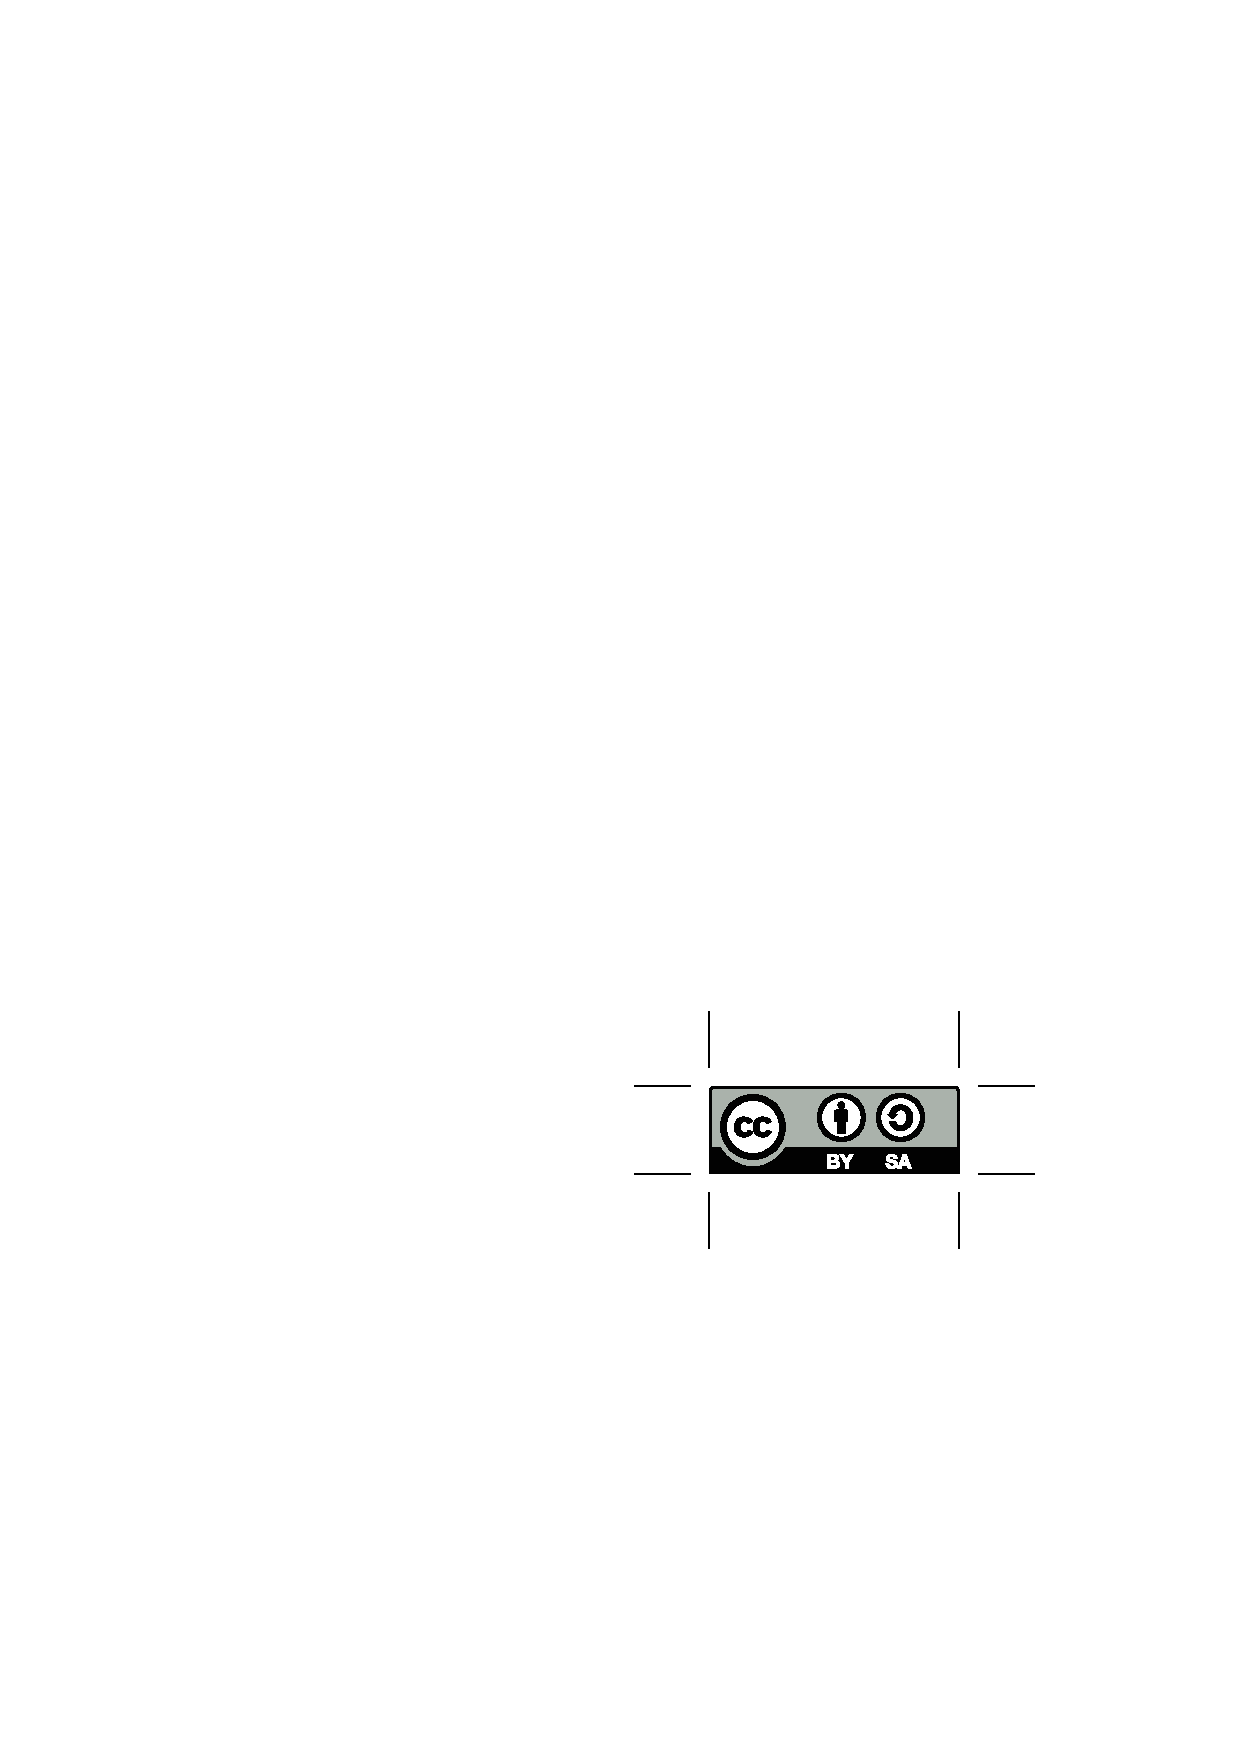
\includegraphics[scale=0.5]{pics/by-sa}
\vspace*{1mm}
\\
\hbox{\parbox{1\textwidth}
{This work is licensed under CC BY-SA 4.0.
To view a copy of this license, visit
\texttt{https://creativecommons.org/licenses/by-sa/4.0}}}}


\thispagestyle{empty}
\newpage

\tableofcontents

\vfill


\begin{figure}[h!]
\centering
\begin{tikzpicture}[->,>=stealth',shorten >=1pt,auto,scale=.25,
  thick,main node/.style={circle,draw,font=\sffamily\bfseries,minimum size=8mm}]

  \node[main node] (1) at (0,0) {\ref{chap:curves-def}};
  \node[main node] (2) at (3,-5) {\ref{chap:length}};
  \node[main node] (3) at (6,-10) {\ref{chap:curve-curvature}};
  \node[main node] (4) at (9,-5) {\ref{chap:poly}};
  \node[main node] (5) at (9,-15) {\ref{chap:torsion}};
  \node[main node] (6) at (12,-10) {\ref{chap:signed-curvature}};
  \node[main node] (7) at (15,-15) {\ref{chap:supporting-curves}};
  \node[main node] (8) at (18,0) {\ref{chap:surfaces-def}};
  \node[main node] (9) at (15,-5) {\ref{chap:first-order}};
  \node[main node] (10) at (18,-10) {\ref{chap:surface-curvature}};
  \node[main node] (11) at (21,-15) {\ref{chap:Curves in a surface}};  
  \node[main node] (12) at (18,-20) {\ref{chap:surface-support}};
  \node[main node] (13) at (21,-5) {\ref{chap:shortest}};
  \node[main node] (14) at (24,-10) {\ref{chap:geodesics}};
  \node[main node] (15) at (27,-15) {\ref{chap:parallel-transport}};
  \node[main node] (16) at (33,-15) {\ref{chap:gauss-bonnet}};
  \node[main node] (17) at (30,-10) {\ref{chap:semigeodesic}};
  \node[main node] (18) at (36,-10) {\ref{chap:comparison}};
  
  \path[every node/.style={font=\sffamily\small}]
   (1) edge node{}(2)
   (2) edge node{}(3)
   (3) edge node{}(5)
   (3) edge node{}(4)
   (3) edge node{}(6)
   (4) edge[dashed] node{}(6)
   (6) edge node{}(7)
   (6) edge node{}(10)
   (7) edge node{}(12)
   (8) edge node{}(9)
   (8) edge node{}(13)
   (9) edge node{}(10)
   (10) edge node{}(11)
   (11) edge node{}(12)
   (10) edge node{}(14)
   (13) edge node{}(14)
   (14) edge node{}(15)   
   (14) edge[bend left= 15] node{}(17)
(17) edge[dashed, bend left= 15] node{}(14)
   (15) edge node{}(16)
   (16) edge[dashed] node{}(18)
   (17) edge[dashed] node{}(15)
   (17) edge[dashed] node{}(16)
   (17) edge node{}(18);
\end{tikzpicture}
\end{figure}

\vfill

\newpage
%\phantomsection
\chapter*{Preface}
\addcontentsline{toc}{part}{Preface}
\thispagestyle{myheadings}
\markboth{PREFACE}{PREFACE}

These notes are designed for those who either plan to work in differential geometry,
or at least want to have a good reason \textit{not} to do~it.
It should be more than sufficient for a semester-long course. 

Differential geometry exploits several branches of mathematics, including 
real analysis, 
measure theory,
calculus of variations,
differential equations,
elementary and convex geometry,
topology, and more.
This subject is wide even at the beginning. 
For that reason, it is fun and painful both to teach and to study.

In this book, we discuss smooth curves and surfaces --- the main gate to differential geometry.
This subject provides a collection of examples and ideas critical for further study.
It is wise to become a master in this subject before making further steps --- there is no need to rush.

We give a general overview of the subject, keeping it
problem-centered,
elementary, 
visual, 
and virtually rigorous; we allow gaps that belong to other branches of mathematics, most of these subjects discussed briefly in the preliminaries.

We focus on the techniques that are absolutely essential for further study.
For  that reason we omit a number of topics that are traditionally included in the introductory texts;
for example, we almost do not touch 
minimal surfaces
and the Peterson--Codazzi formulas.
%(In an ideal world, we could also remove the chapter about torsion, but we decided to yield to tradition this once.) 

At the same time, we get to applications that are not in the scope of typical introductory texts.
 
The first example is the theorem of Vladimir Ionin and Herman Pestov about the Moon in a puddle (\ref{thm:moon-orginal}).
This theorem might be the simplest meaningful example of the so-called {}\emph{local to global theorems} which lies in the heart of differential geometry;
for that reason, it is a good answer to the main question of this book --- ``What is differential geometry?''.

Other examples include the theorem of Sergei Bernstein on saddle graphs (\ref{thm:bernshtein}) and the theorem of Stephan Cohn-Vossen
on a two-sided infinite geodesic (\ref{thm:cohn-vossen}).

These notes are based on the lectures given at the MASS program (Mathematics Advanced Study Semesters at Pennsylvania State University) in the fall of 2018.
Many of the topics were presented by Yurii Burago in his lectures teaching the first author at Leningrad University.
We extensively used textbooks
by Wilhelm Blaschke and Kurt Leichtweiss~\cite{blaschke-leichtweiss},
by Aleksei Chernavskii~\cite{chernavsky},
and by Victor Toponogov~\cite{toponogov-book}, and also the lecture notes of Sergei Ivanov \cite{ivanov};
many advanced exercises are taken from \cite{petrunin2020}.
The last chapter is based on the introductory material in the book by Stephanie Alexander, Vitali Kapovitch, and the first author~\cite{alexander-kapovitch-petrunin2027}.
We want to thank
Stephanie Alexander,
Yurii Burago, 
Berk Ceylan,
Nina Lebedeva,
Alexander Lytchak,
Benjamin McKay,
and all the students in our class
for their help.

The present work is partially supported by NSF grant DMS-2005279
and by the Simons Foundation under grant \#584781.

\begin{flushright}
Anton Petrunin and\\
Sergio Zamora Barrera.
\end{flushright}




